\documentclass{article}
\usepackage[utf8]{inputenc}
\usepackage{hyperref}
\usepackage{natbib}
\usepackage{graphicx}



\hypersetup{
    colorlinks=true,
    linkcolor=blue,
}

\begin{document}

\title{Tn-Seq Analysis Protocol}
\author{Margaret-Mary Antonio \& Katherine Maia McCoy, Tim van Opijnen}
\date{December 10th, 2016}
\maketitle

\newpage

\section{An Overview of Tn-Seq}

\vspace{2 mm}

\noindent
Tn-Seq is a method of determining quantitative fitnesses of bacterial genes. This manual is not meant to describe it in full, only how to analyze the sequencing data it produces. If you are unfamiliar with Tn-Seq or require a refresher, several scientific papers (\href{http://www.nature.com/nmeth/journal/v6/n10/abs/nmeth.1377.html}{1,} \href{http://www.nature.com/nrmicro/journal/v11/n7/abs/nrmicro3033.html}{2,} \href{http://www.ncbi.nlm.nih.gov/pmc/articles/PMC3514683/}{3,} \href{http://journals.plos.org/plospathogens/article?id=10.1371/journal.ppat.1005869}{4}) have been published with detailed explanations.

\vspace{5 mm}

\noindent
To begin, the tools and steps you must use on your data depend on how the sequences were prepared. We review sample preparation in \textbf{Figure 1.} 

\vspace{7 mm}

\noindent
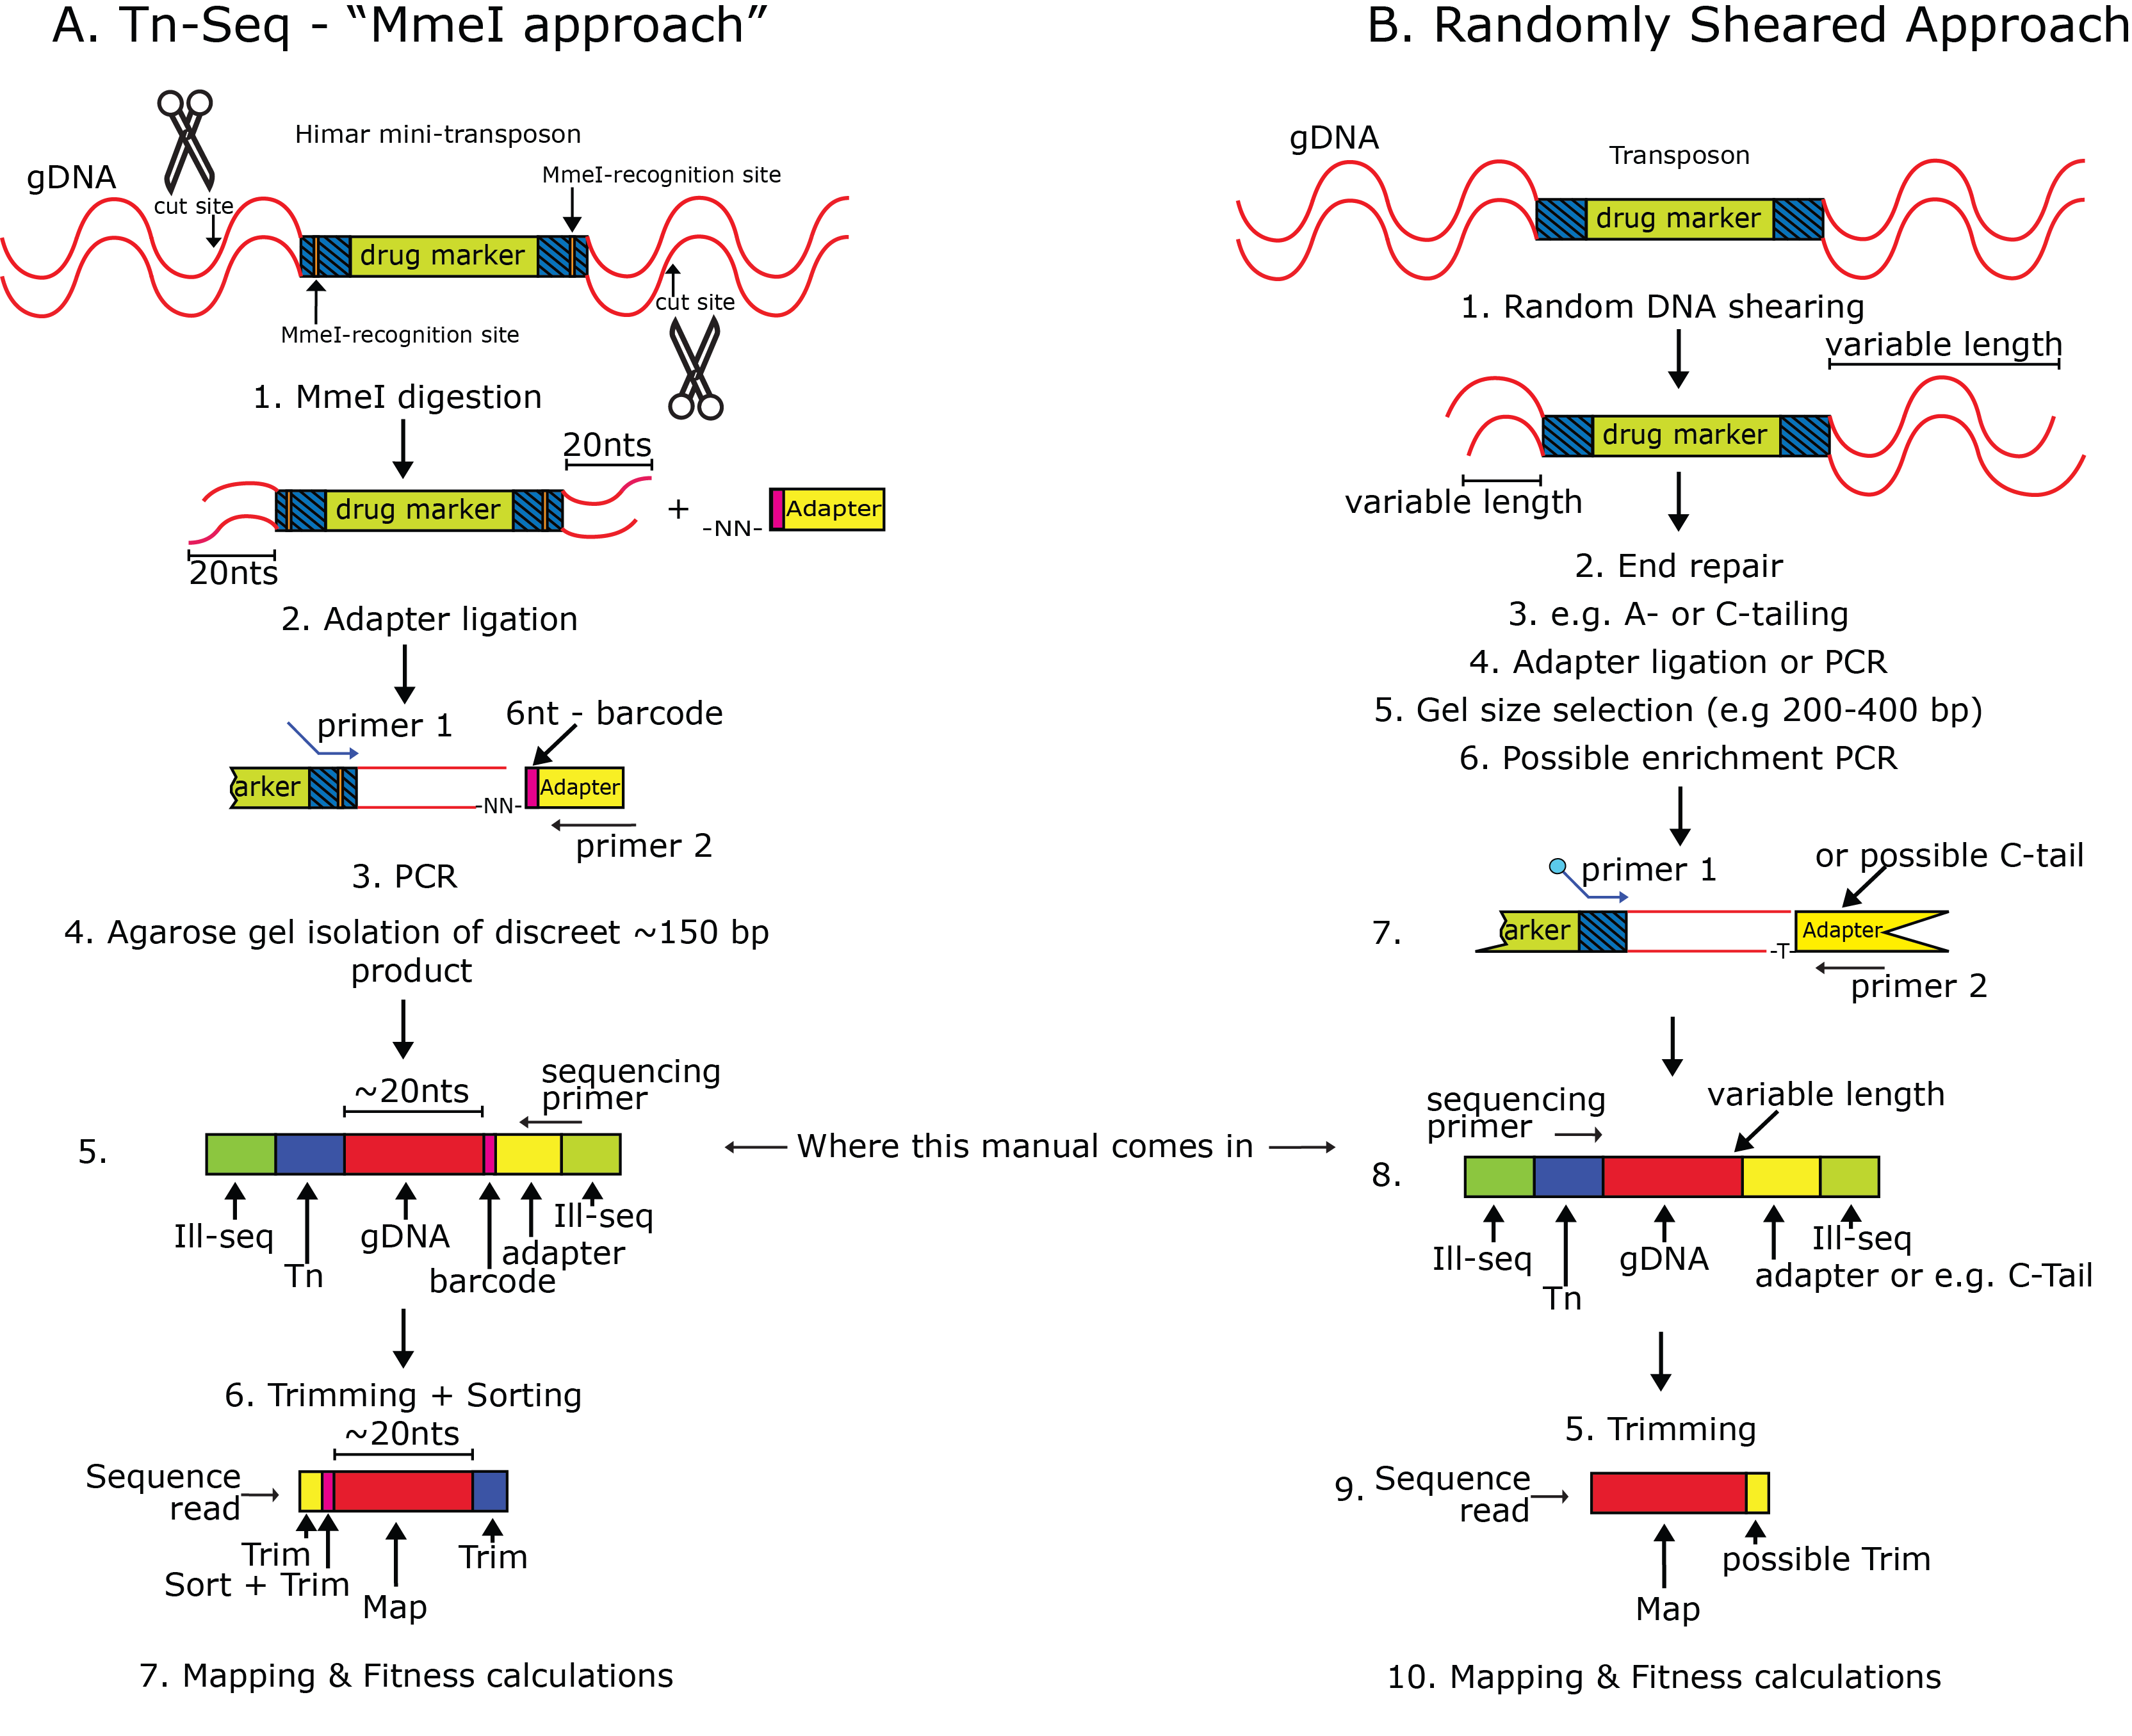
\includegraphics[scale=0.87]{SeqProdOverview.png}

\noindent
\textbf{Figure 1.} An overview of the two main approaches to Tn-Seq sample preparation, which both end in products able to be sequenced on an Illumina sequencer. \textbf{A.)} Shows the different steps in the \href{http://www.nature.com/nmeth/journal/v6/n10/abs/nmeth.1377.html}{MmeI Tn-Seq procedure}, which uses MmeI digestion. It generates a PCR product of approximately 150bp, with two flanking sequences  essential to enable Illumina sequencing (in green), a small piece of the transposon sequence (in blue), approximately 20nts of bacterial genomic DNA (gDNA; in red), and the adapter sequence (in yellow), which also contains a 6nt barcode to enable multiplexing (in pink). Note that in this approach sequencing starts from the sequencing primer on the right then reads into the barcode, the gDNA, and finally the transposon. \textbf{B.)} Shows the randomly sheared approach where gDNA is randomly sheared,  so that the product to be sequenced has a variable length. This means it is not clear how large the gDNA fragment is; sequencing starts from the transposon side, reads into the gDNA, and depending on the size of the gDNA may read into the adapter or C-tail.

\vspace{5 mm}

\noindent
After the reads described in Figure 1 are sequenced, they must be computationally analyzed (Fig 2). The first section of analysis is the "Data Prep", in which all non-genomic parts of the sequences are removed and the genomic data is mapped to discover the location of each read. The second section is the "Fitness Analysis", in which the differences in mapped genomic data between an initial time point and a second time point are used to calculate the fitness of various insertions then aggregate them by gene (If you're unfamiliar with the concept of a fitness calculation, see the papers linked at the start). Finally, the third section is "Comparative Analyses \& Other Tools" - these optional analyses / tools let you compare and visualize your fitness data in various useful ways.

\noindent
\includegraphics[scale=0.14]{tnseq_workflow.png}

\noindent
\textbf{Figure 2.} An overview of the various steps of Tn-Seq Data Analysis. Data is trimmed of its non-genomic segments and mapped, has its genomic fitness calculated, and finally can be examined by an array of useful tools.

\newpage
\section{The Files You'll Need}
\label{sec:files}


\noindent
The data you'll need are as follow:

\begin{itemize}
\item Your sequencing reads in \href{http://maq.sourceforge.net/fastq.shtml}{fastq format}. These files should end in .fastq and look like this:

\end{itemize}

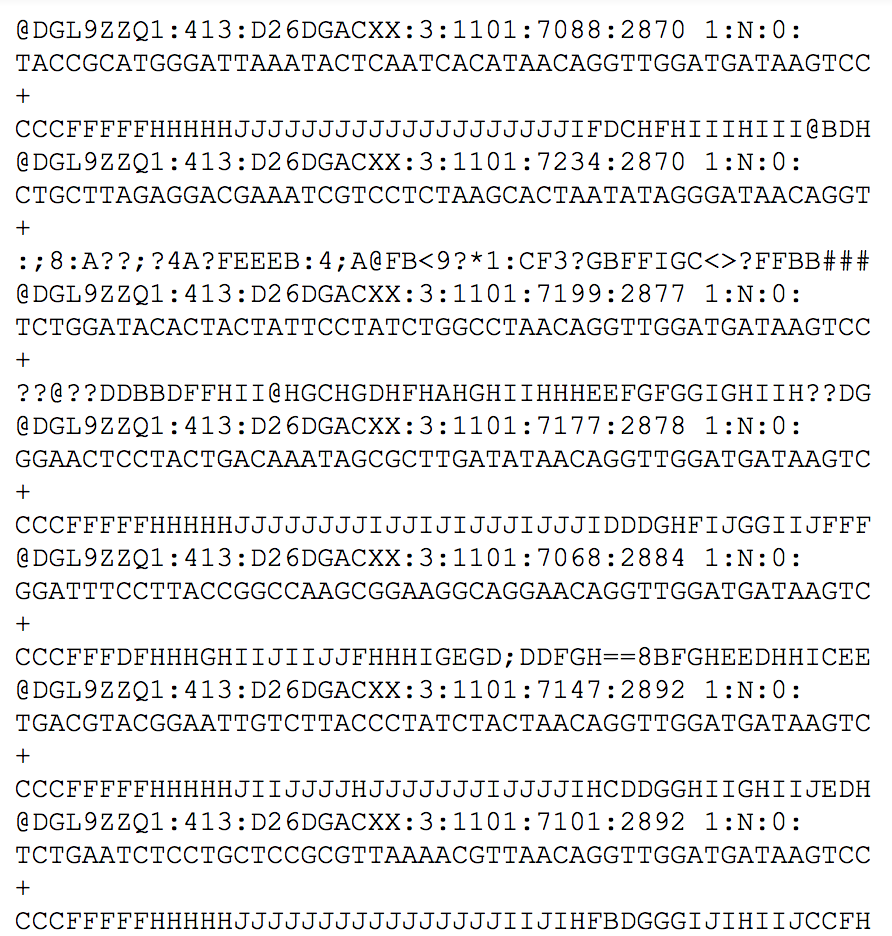
\includegraphics[scale=0.5]{fastq.jpg}

\begin{itemize}

\item Your expansion factors, which are determined experimentally. You divide the number of bacteria you end with by the number you started with; to calculate this in vitro you could plate appropriate dilutions of your starting and cultures then measure their number of Colony Forming Units (CFUs), for instance. In vivo is a bit more complicated, and a reasonable estimation often works as well, but see \href{http://www.ncbi.nlm.nih.gov/pmc/articles/PMC3514683/}{this link} for how you might experimentally determine in vivo growth rates and expansion factors. 

\end{itemize}

\begin{itemize}

\item \href{http://hannonlab.cshl.edu/fastx_toolkit/commandline.html#fastx_barcode_splitter_usage}{Barcode files}, if you used any to differentiate between your different conditions. Make these by hand; give each barcode a line which consists of whatever you'd like th name it, a tab, and its sequence. We strongly recommend putting your expansion factors in their relevant barcode names, for easy identification. These files should end in .txt and look like this:

\end{itemize}

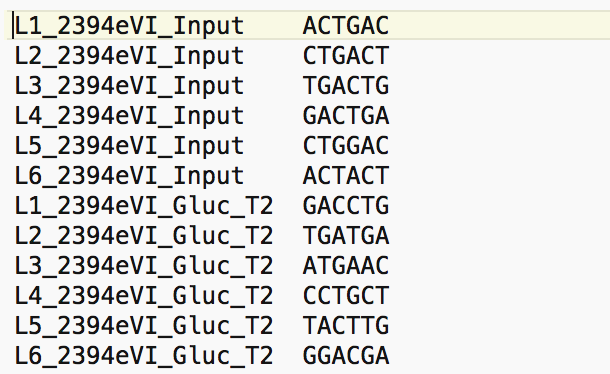
\includegraphics[scale=0.5]{barcode.png}

\begin{itemize}

\item If you are using the MmeI Tn-Seq approach, four additional barcode files which describe the end of the MmeI transposon sequence. (As shown in Fig 1, there is a variable region of adaptor DNA in each read, and these barcodes allow you to identify then trim it off.) They should end in .txt, have one line each, and are exactly as follows:

\end{itemize}

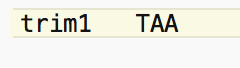
\includegraphics[scale=0.5]{transbc1.png}

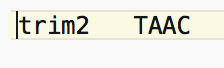
\includegraphics[scale=0.5]{transbc2.png}

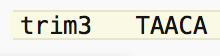
\includegraphics[scale=0.5]{transbc3.png}

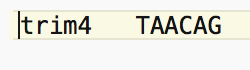
\includegraphics[scale=0.5]{transbc4.png}

\begin{itemize}

\item Genbank files / fasta genome sequences for each strain you're analyzing, whcih can be found on NCBI by searching for each strain under the Genome section. These files should end in .gbk and .fasta respectively, and look like this:

\end{itemize}

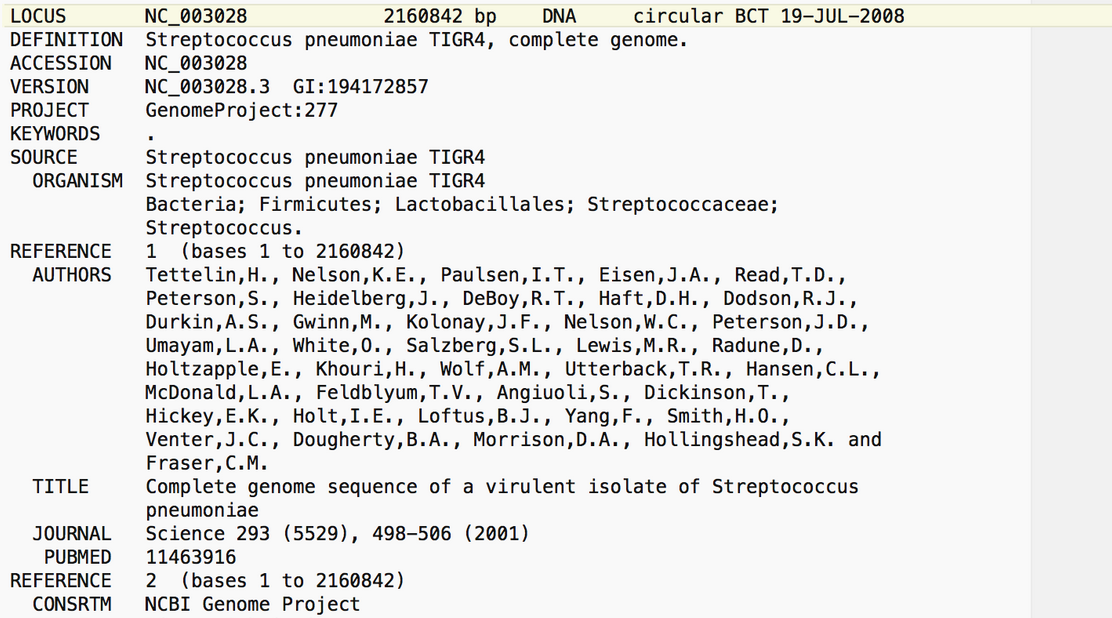
\includegraphics[scale=0.5]{gbk.png}

\vspace{2 mm}

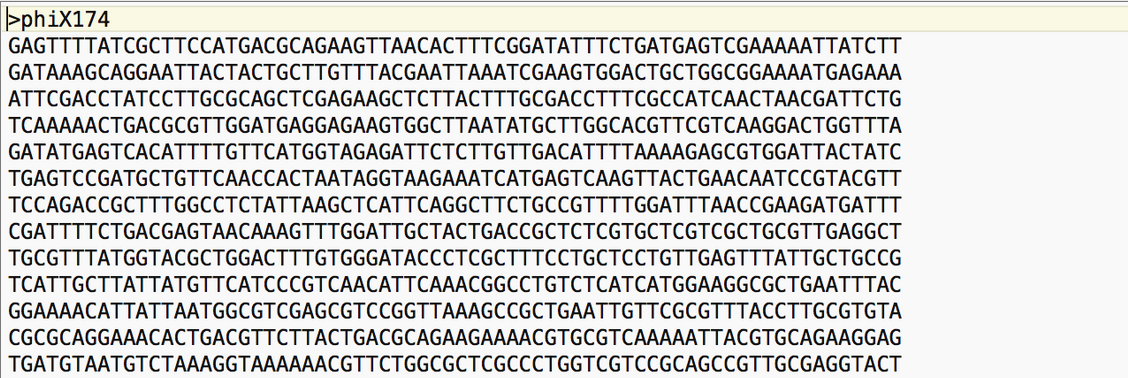
\includegraphics[scale=0.5]{fasta.png}

\begin{itemize}

\item Normalization files for each strain, which are txt files containing all "normalization genes", one per line. Normalization genes are those that should have no effect on fitness when disrupted, and you can generate normalization files yourself by looking through a strain's genbank file and recording all transposon genes, pseudogenes, and degenerate genes - or generally include any gene that you know does not have an effect on fitness. However, this file is not essential and if it is not available or you don't want to compile it, it is often OK to run the analysis without it. These files should end in .txt.

\end{itemize}

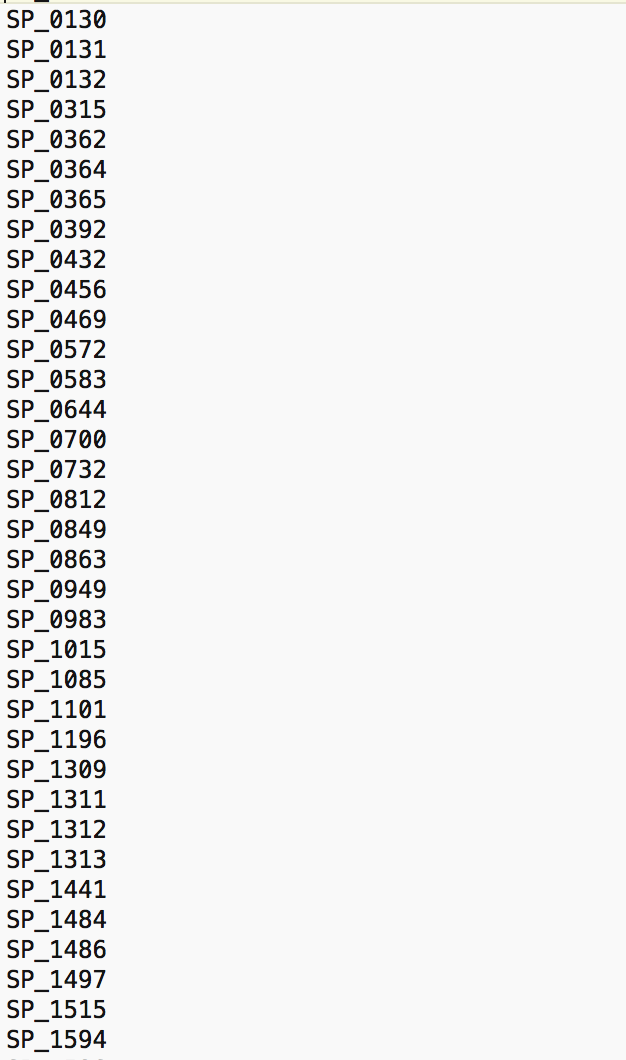
\includegraphics[scale=0.5]{normalization.png}


\vspace{5 mm}

\noindent
Finally, if you'd rather run our tools manually through the command line, rather than automatically through Galaxy, you can skip down to command line instructions \hyperref[sec:command]{here}. Otherwise, continue on for the Galaxy instructions.

\newpage

























\section{Analysis via Galaxy}

\vspace{2 mm}

\noindent
If you have never used Galaxy or our tools before, an easy tutorial on how to set Galaxy up can be found \href{https://wiki.galaxyproject.org/Admin/GetGalaxy}{here}, how to upload files is described \href{https://wiki.galaxyproject.org/Admin/DataLibraries/UploadingLibraryFiles}{here}, and our custom tools can all be found and installed through \href{https://wiki.galaxyproject.org/Admin/Tools/AddToolFromToolShedTutorial}{the Galaxy toolshed}. You can find them by searching for their names in the toolshed: 

\begin{itemize}
\item enhanced\_bowtie\_mapper
\item fastq\_collapser
\item calculate\_fitnesses
\item and aggregate\_fitnesses

\end{itemize}


\vspace{2 mm}

\noindent
As described in Figure 1, there are three main parts to the analysis. The first, the Data Prep, varies depending on your type of data. If you prepared your samples with the MmeI Tn-Seq method, you'll use the \hyperref[subsec:mmei]{MmeI Tn-Seq Prep}. If you prepared your samples with a random shearing method, you'll use the \hyperref[subsec:random]{Randomly Sheared Tn-Seq Prep}. If you prepared your samples some other way, you can follow this generalized data prep protocol for making your own workflow via Galaxy's \href{https://wiki.galaxyproject.org/Learn/AdvancedWorkflow}{workflow editor}:

\begin{itemize}
\item Split data by experimental condition barcodes, if any, using the fastx barcode splitter.
\item Remove all non-genomic DNA using a tool like the fastq trimmer.
\item Filter reads by quality using the fastq quality splitter, if you like.
\item Map reads in Bowtie. We recommend using most standard flags, with the following modifications: use best, try hard, discard reads mapping to multiple locations, and have the output be in map format (as the calc\_fit tool only takes inputs in this format). The number of allowed mismatches can be fiddled with, but should be relatively low to prevent false mapping.

\end{itemize}

\vspace{2mm}

\noindent
After the data prep, everything else is done in the same way. The fitness analysis is done with the \hyperref[subsec:fitness]{Calculate / Aggregate Fitness} Workflow, and the \hyperref[subsec:comparative]{Comparative Analyses \& Other Tools} can then be used to sort through and visualize your fitness data.

\newpage

\subsection{MmeI Tn-Seq Prep}
\label{subsec:mmei}

\vspace{2 mm}

Download links: \href{https://github.com/vanOpijnenLab/magenta-p2/blob/master/workflows/Galaxy-Workflow-MmeI_Tn-Seq_Prep_Pt.1.ga}{Pt 1}, \href{https://github.com/vanOpijnenLab/magenta-p2/blob/master/workflows/Galaxy-Workflow-MmeI_Tn-Seq_Prep_Pt.2.ga}{Pt 2}, and \href{https://github.com/vanOpijnenLab/magenta-p2/blob/master/workflows/Galaxy-Workflow-MmeI_Tn-Seq_Prep_Pt.3.ga}{Pt 3}
\vspace{5 mm}

\noindent
    This prep assumes a 50nt read, as described in Fig. 1 A), with its first 9 nucleotides from an adaptor, the next six from its barcode, the next 15 to 18 from genomic DNA, and the last 20 to 23 from its transposon. In Part 1 it trims the first 9 and last 17, then splits by the potential segments of transposon DNA (TAA, TAAC, TAACA, or TAACAG) left on its end using the barcode splitter. In part 2 it trims that remaining transposon DNA, concatinates the files back into one, and splits by experimental barcode with the barcode splitter. In Part 3 it trims the barcodes from the reads and puts the barcode names in the file names so that they're labeled by experimental condition, filters the reads, collapses them, and maps them to the genome provided.

\vspace{5 mm}
\noindent
\textbf{Part 1: trim \& split by trailing transposon sequence}

\begin{itemize}

\item Navigate to the workflow tab, click on the “Standard Tn-Seq Prep Pt.1” workflow, and select “Run”. You should see a workflow with these steps:

\end{itemize}

\vspace{5 mm}

\noindent
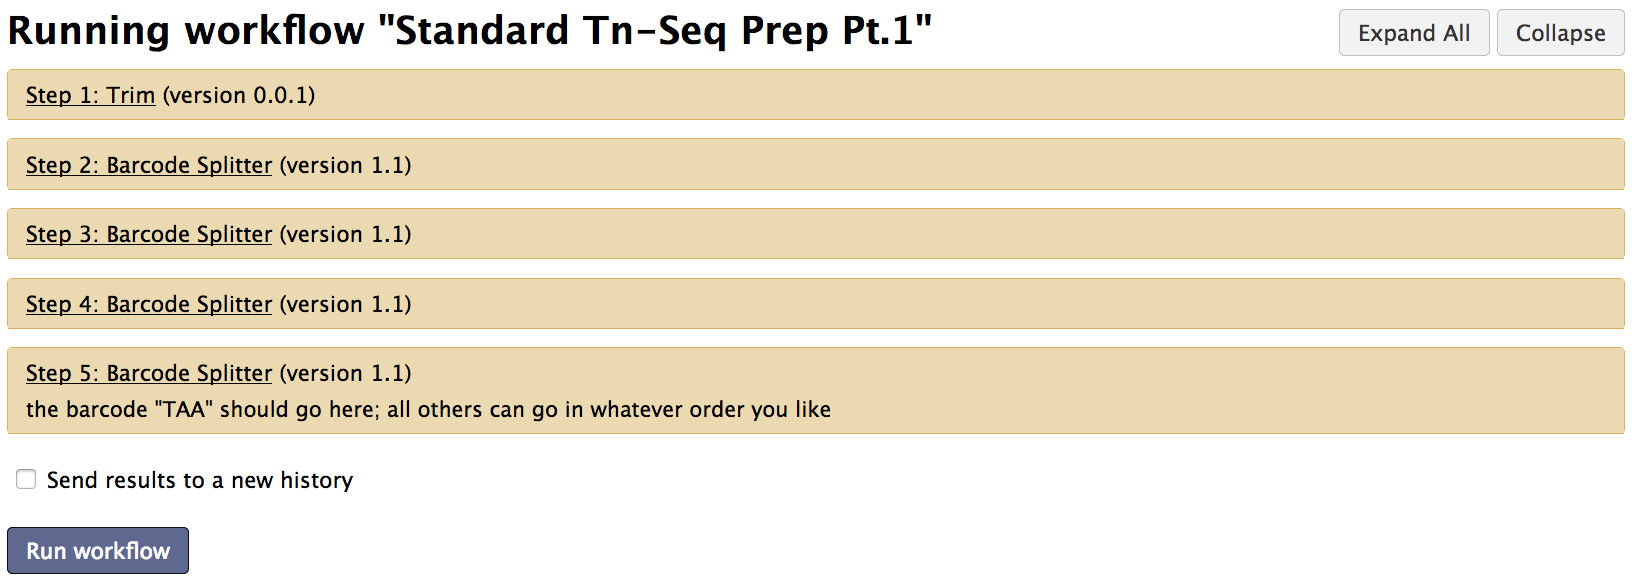
\includegraphics[scale=0.5]{StandPrep1.png}

\vspace{5 mm}

\begin{itemize}

\item Select your FASTQ file under “this dataset” in “Step 1: Trim”. The default settings will trim of the first 9 and the last 17nts.
\item Select your four transposon sequence barcode files in Steps 2 through 5, one per step. Note that these transposon-endings are entered as "barcodes" in the workflow, but they are not your experimental barcodes, just transposon ends the tool searches for like barcodes. They can go in whichever order you wish, except that the "trim1" barcode (finds sequences ending in TAA) should go under Step 5, which allows for 0 mismatches, because it is only 3 bp long so even a single mismatch is too loose a constraint.
\item Press “Run workflow”, and wait for the workflow to finish running.

\end{itemize}

\vspace{5 mm}

\noindent
\textbf{Part 2: trim trailing transposon sequence, concatenate files together, and split by barcode}

\vspace{5 mm}

\begin{itemize}

\item Navigate to the workflow tab, click on the “Standard Tn-Seq Prep Pt.2” workflow, and select “Run”. You should see a workflow with these steps:

\end{itemize}

\vspace{5 mm}

\noindent
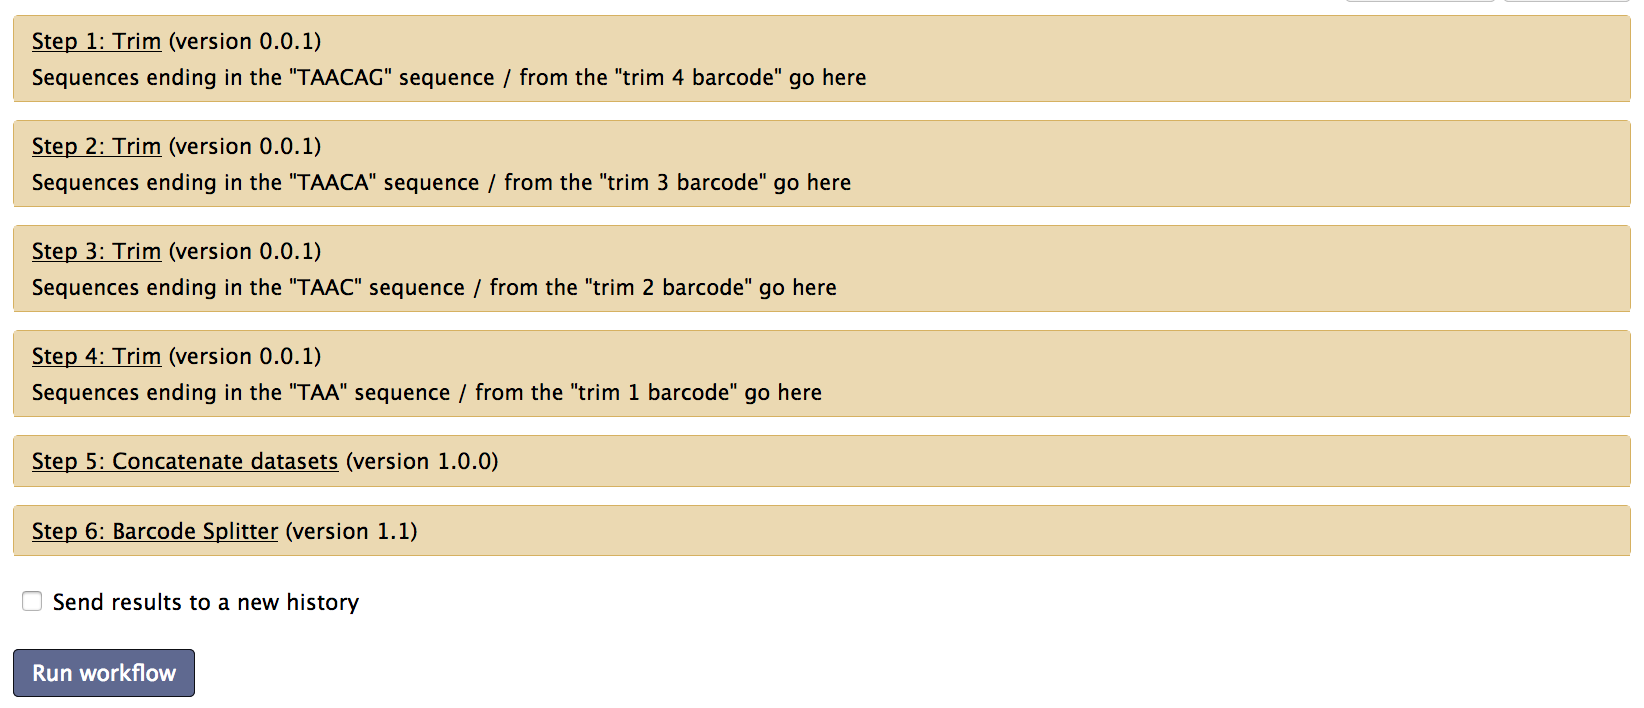
\includegraphics[scale=0.5]{StandPrep2.png}

\vspace{5 mm}

\begin{itemize}

\item Select your trim4 barcode-split file under “this dataset” for “Step 1: Trim” (the step with “-4” under “Remove everything from this position to the end”).
\item Select your trim3 barcode-split file under “this dataset” for “Step 2: Trim” (the step with “-3” under “Remove everything from this position to the end”).
\item Select your trim2 barcode-split file under “this dataset” for “Step 3: Trim” (the step with “-1” under “Remove everything from this position to the end”). 
\item Select your trim1 barcode-split file under “this dataset” for “Step 4: Trim” (the step with “-2” under “Remove everything from this position to the end”).
\item Select your barcode file under “Barcodes to use” in “Step 6: Barcode Splitter”. These should be the barcodes identifying which experimental condition each read is from.
\item Press “Run workflow”, and wait for the workflow to finish running.
\item Refresh your history and make a list out of the resulting files to send into the next workflow, via the “operations on multiple datasets” button. The button looks like this and is in Galaxy's history sidebar:

\end{itemize}


\includegraphics[scale=1.0]{opbutton.png}

\vspace{5 mm}

\noindent
\textbf{Part 3: trim barcode, filter reads by quality, collapse reads, and map them}
\vspace{5 mm}

\begin{itemize}

\item Navigate to the workflow tab, click on the “Standard Tn-Seq Prep Pt.3” workflow, and select “Run”. You should see a workflow with these steps:

\end{itemize}

\vspace{5 mm}

\noindent
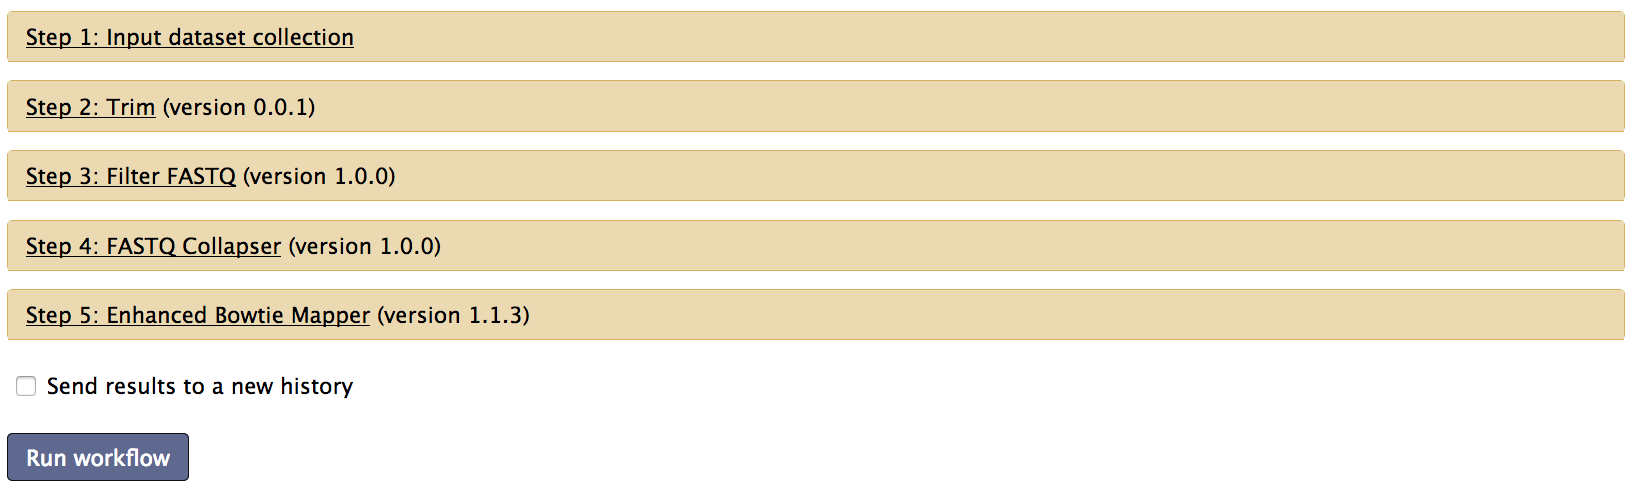
\includegraphics[scale=0.5]{StandPrep3.png}

\vspace{5 mm}

\begin{itemize}

\item Under “Step 5: Map with Bowtie for Illumina”, select your fasta genome under “Select the reference genome”.
\item Press “Run workflow”, and wait for the workflow to finish running.

\end{itemize}

\newpage

\subsection{Randomly Sheared Tn-Seq Prep}
\label{subsec:random}

\vspace{2 mm}

Download \href{https://github.com/vanOpijnenLab/magenta-p2/blob/master/workflows/Randomly%20Sheared%20Data%20Prep.ga}{link}

\vspace{5 mm}

\noindent
As described in Fig. 1 B), another method to prepare your Tn-Seq sample involves DNA shearing and ligating on C-tails. This prep assumes a 50nt read of genomic DNA followed by a C-tail, of variable length due to the randomness of the shearing. It removes the C-tail from the end with Cutadapt, grooms the reads, filters them for quality, collapses them, and maps them. If your reads were prepared in this manner but also had barcodes, you should use the barcode splitter tool to separate them by barcode first.

\vspace{5 mm}

\begin{itemize}

\item First make a list out of all the sequence files you want to analyze, via the “operations on multiple datasets” button. The button looks like this and is in Galaxy's history sidebar:

\end{itemize}


\includegraphics[scale=1.0]{opbutton.png}

\begin{itemize}

\item Next navigate to the workflow tab, click on the “Randomly Sheared Data Prep” workflow, and select “Run”. You should see a workflow with these steps:

\end{itemize}

\vspace{5 mm}

\noindent
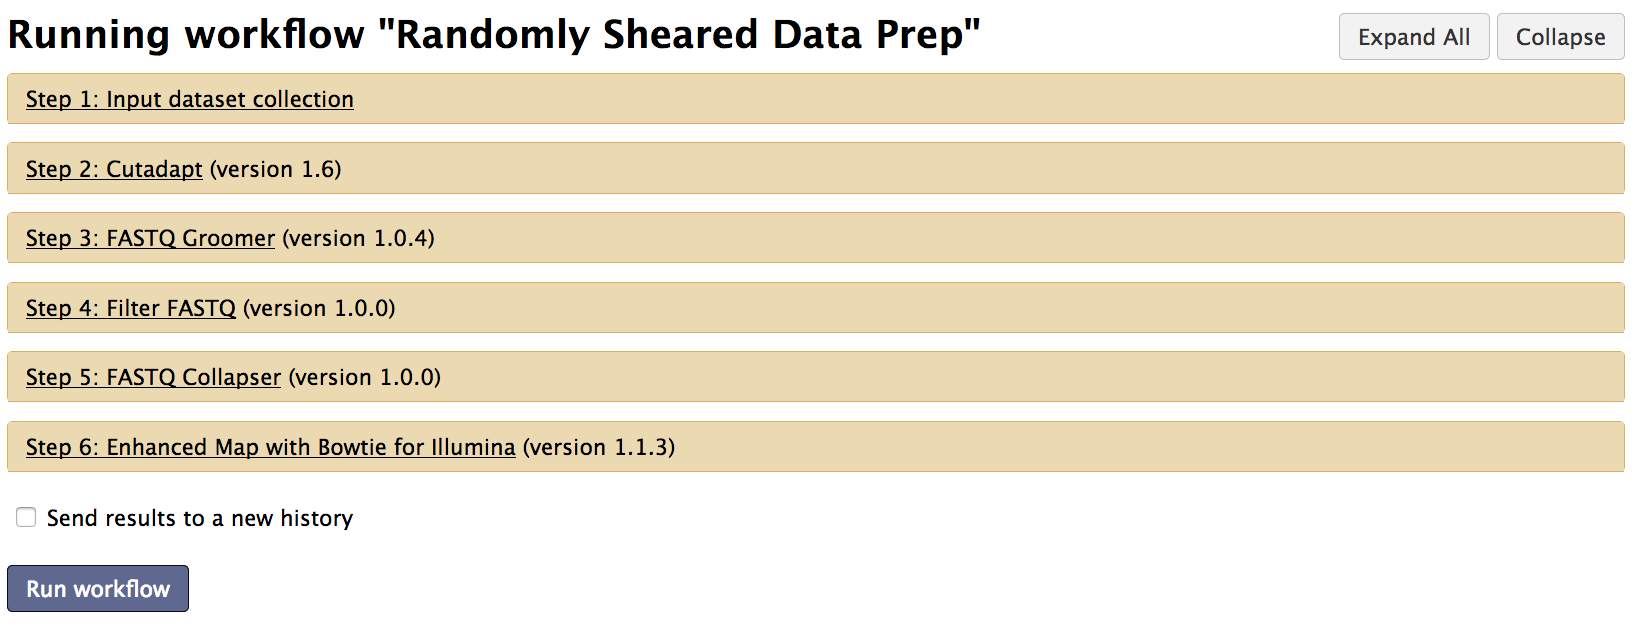
\includegraphics[scale=0.5]{Random.png}

\vspace{5 mm}

\begin{itemize}

\item Enter the list of your files under “Step 1: Input dataset collection" 
\item At “Step 6: Map with Bowtie for Illumina”, select your fasta genome under “Select the reference genome”. Make sure this is your .fa file not your .gbk file.
\item Press “Run workflow”, and wait for the workflow to finish running.

\end{itemize}

\newpage

\subsection{Tn-Seq Fitness Analysis}
\label{subsec:fitness}

Download \href{https://github.com/vanOpijnenLab/magenta-p2/blob/master/workflows/Calculate%20Fitnesses%20:%20Aggregate%20Fitnesses.ga}{link}

\vspace{2 mm}
\noindent
This workflow first calculates fitnesses for each insertion in the genome, then aggregates them by gene. You can also use the aggregate tool on multiple Calculate Fitness output files to make a 'super' aggregate file, which calculates fitness of genes by averaging fitness of all insertions across multiple libraries. Note that this workflow cannot be run in batch, because each run requires a unique expansion read, so repeat the below steps for each time 2 condition you want to analyze.

\begin{itemize}

\item Navigate to the workflow tab, click on the “Calculate / Aggregate Fitness” workflow, and select “Run”. You should see a workflow with these steps:

\end{itemize}

\vspace{5 mm}

\noindent
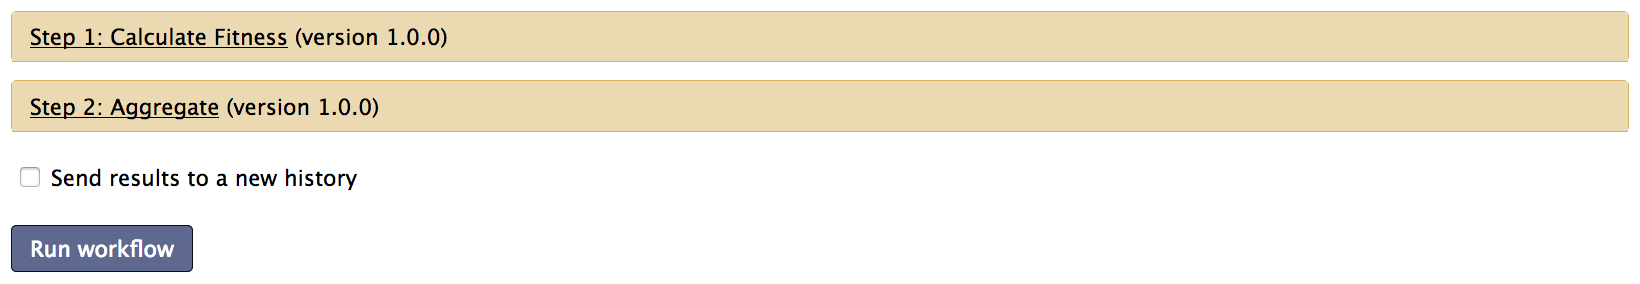
\includegraphics[scale=0.5]{CalcAgg.png}

\vspace{5 mm}

\begin{itemize}
\item In “Step 1: Calculate Fitness”, select your map files from t1, map files from t2, GenBank reference genome, and normalization genes under the corresponding headers. 
\item In “Step 1: Calculate Fitness”, click the edit symbol under “Expansion Factor” and edit that value to your time 2 sample’s expansion factor, in that same step.
\item In “Step 2: Aggregate”, Select your GenBank reference genome under the corresponding header.
\item In “Step 2: Aggregate”, if you’d like to mark certain genes (like say, normalization genes, for reference) chose “Yes” under “Mark certain genes?”. Then chose your normalization genes file or a similarly formatted file as input.
\item Press “Run workflow”, and wait for the workflow to finish running.
\item Once this is done, if you have data from different libraries under the same condition, you can aggregate that data all together (recommended). Do this by navigating to the "Aggregate" tool and using the option to "Insert additional CSV fitness files" as well as selecting "Yes" under "Enter a custom blank count?" as shown below. For the custom blank count, simply average the blank counts of each fitness file you're using, which can be found in its corresponding calc fitness txt file output. Then enter all the fitness files from the same condition, and press “Execute”!

\end{itemize}

\newpage

\subsection{Comparative Analyses \& Other Tools}
\label{subsec:comparative}

[[Margaret's Galaxy notes go here]]

\newpage

\section{Analysis via Command Line}
\label{sec:command}

\vspace{2 mm}

\noindent
If you know a bit of coding, and would rather run our tools through the command line, you may do this. We don't necessarily recommend it, just because it takes much more of the user's time, as jobs must be entered manually via the command line and don't automatically flow into each other like they do in Galaxy. The steps are as follows: 

\vspace{5 mm}

\noindent
1. The Data Prep.

\begin{itemize}

\item Download and install the \href{http://hannonlab.cshl.edu/fastx_toolkit/}{fastx\_toolkit} and  \href{http://bowtie-bio.sourceforge.net/index.shtml}{bowtie}. For more on the usage of the fastx\_toolkit see its \href{http://hannonlab.cshl.edu/fastx_toolkit/commandline.html}{manual}, and for more on Bowtie see its \href{http://bowtie-bio.sourceforge.net/manual.shtml}{manual}.
\item Split data by experimental condition (i.e. barcodes) with fastx barcode splitter and remove all non-genomic DNA (e.g. barcodes) with fastx trimmer. These steps may be done in whatever order best suits your data.
\item Filter reads by quality (e.g. a minimum quality of 8) using fastq quality filter.
\item Collapse reads using fastq collapser.
\item Map reads using Bowtie. We recommend using the following flags: -n 1 (maximum 1 mismatch) --best (Wwether or not to make Bowtie guarantee that reported singleton alignments are 'best' in terms of stratum and quality) -y (try hard) and -m 1 (supress all alignments if more than one can be found)

\end{itemize}

\vspace{5 mm}

\noindent
2. Fitness Analysis

\begin{itemize}

\item Download our \href{https://github.com/vanOpijnenLab/magenta-p2/blob/master/tools/Calculate%20Fitnesses/calc_fitness.py}{calculate\_fitness} tool and our \href{https://github.com/vanOpijnenLab/magenta-p2/blob/master/tools/Aggregate%20Fitnesses/aggregate.py}{aggregate\_fitness} tool. 
\item For every pair of t1/t2 reads, calculate the fitnesses of insertion locations using the calc\_fitness.py. Usage as follows:

\end{itemize}

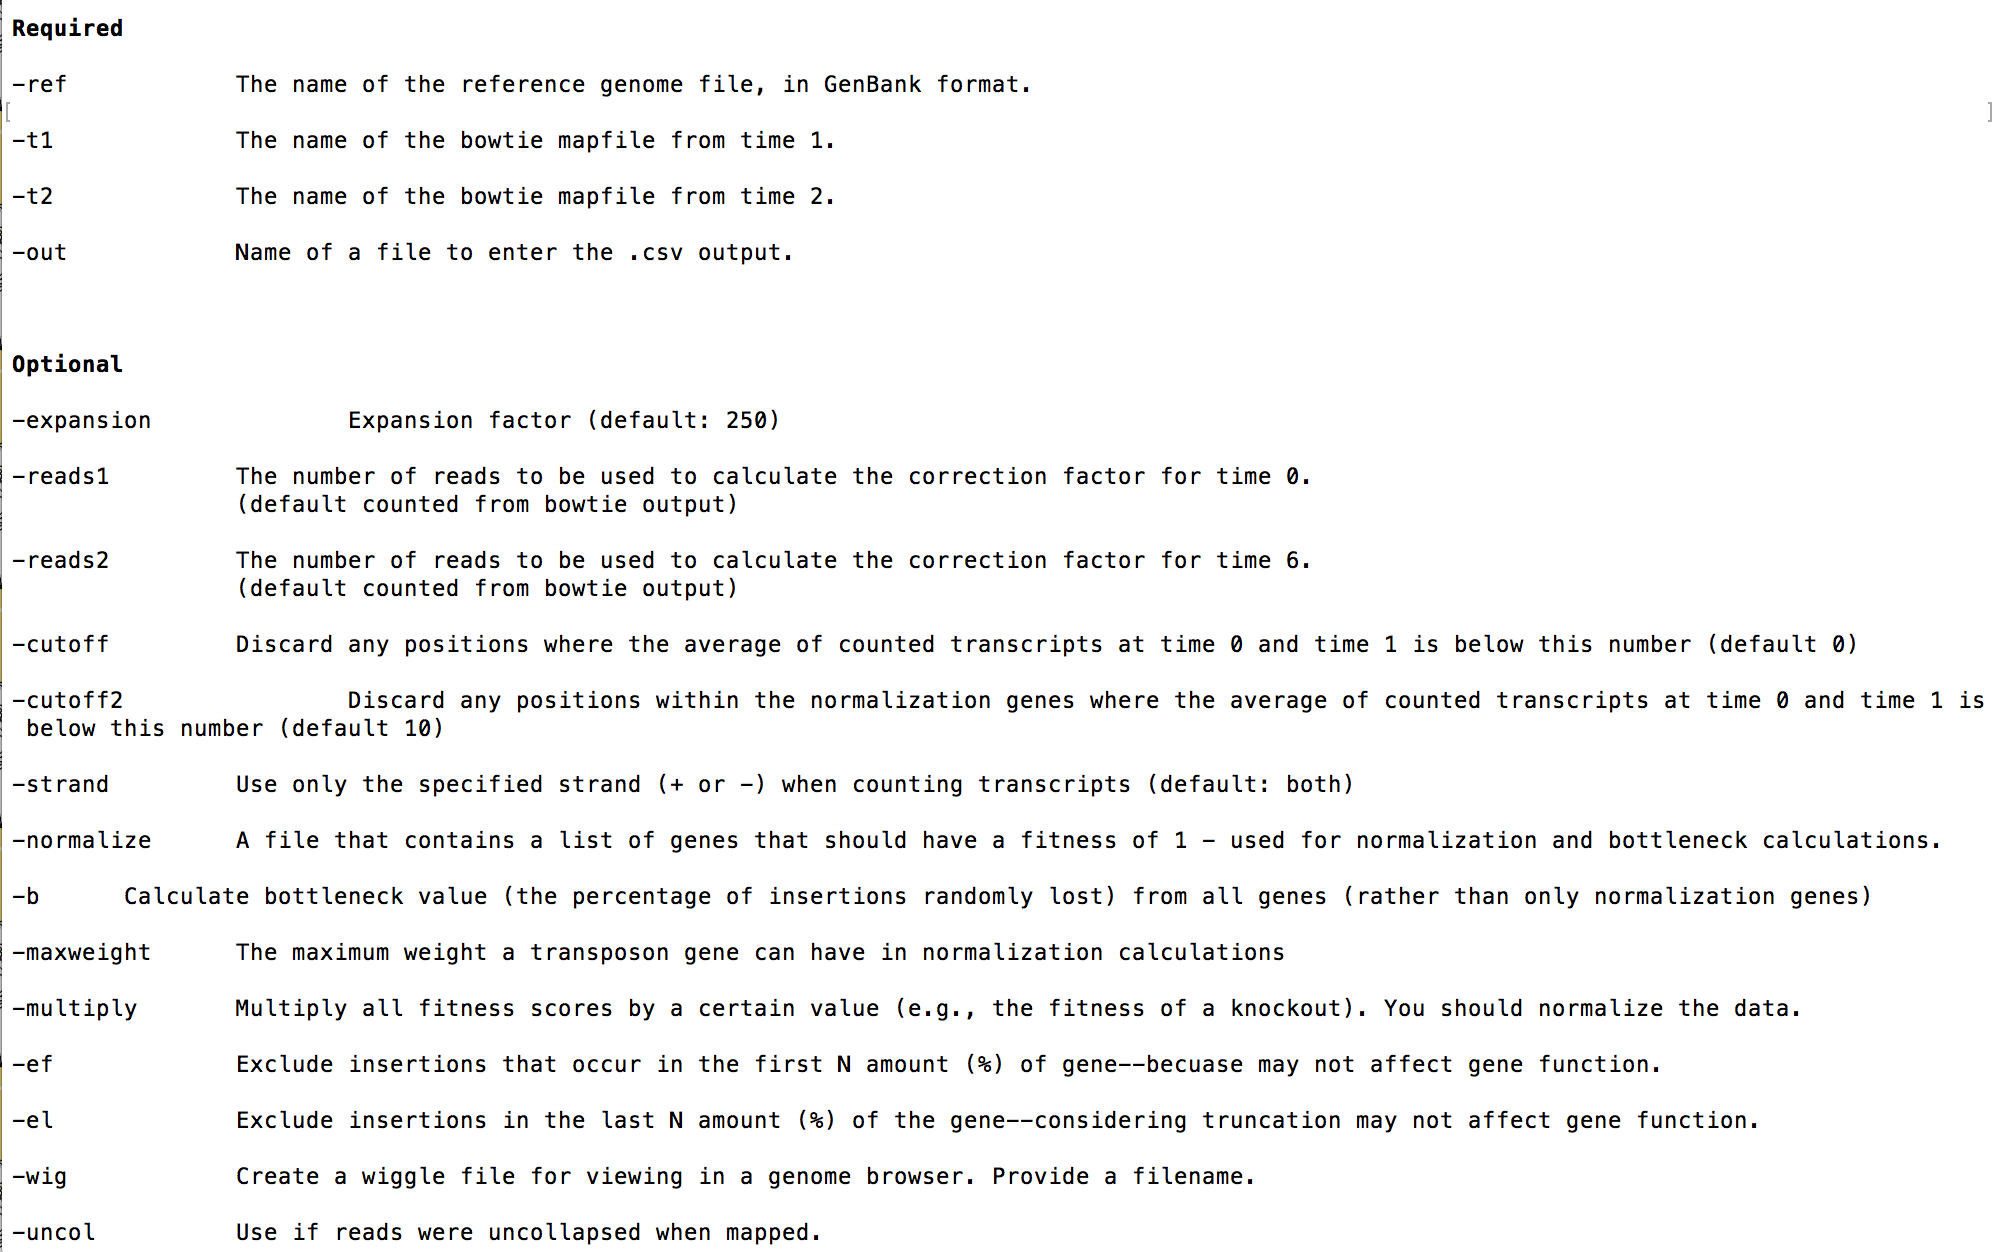
\includegraphics[scale=0.4]{CalcOpts.png}

\begin{itemize}

\item For every csv file calculate\_fitness outputs with the fitnesses of insertion locations, calculate the fitnesses of genes with aggregate.py. Usage as follows:

\end{itemize}

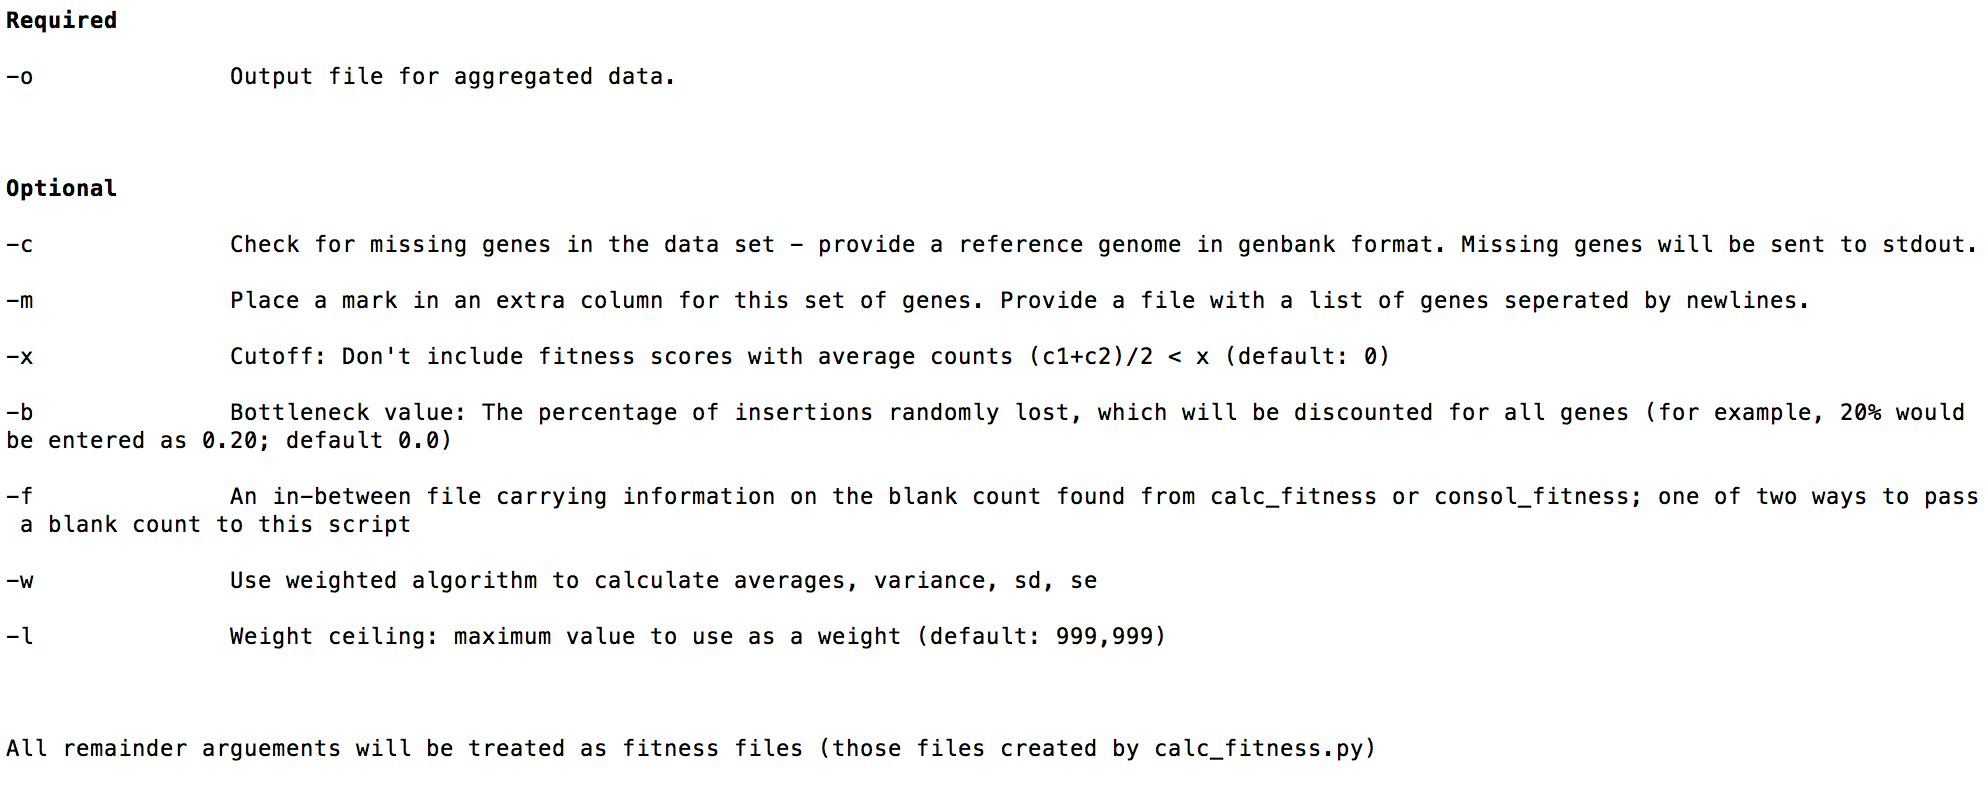
\includegraphics[scale=0.4]{AggOpts.png}

\vspace{5 mm}

\begin{itemize}

\item As described in the aggregate.py usage, you may also input multiple insertion location fitness files, and so make "super aggregate" files that incorporate the data from all your runs. This is highly recommended.

\end{itemize}

\vspace{5 mm}


\noindent
3. Comparative Analyses \& Other Tools

\noindent
[[Margaret's command line documentation should fit in well here - I tried matching my commamd line documentation to her formatting!]]


\end{document}